%!TEX root = ../../Paper.tex

\chapter{Trend Detection on Twitter: Concept}
\label{cha:trend-detection-concept}

\section{Related Work}
\label{sec:related-work}
\todo[inline]{Not sure if this is best place for a twitter description, but the text is good}
Twitter, a popular microblogging service with over 255 million active monthly users\footnote{\url{http://about.twitter.com/company} \accessednote \label{aboutwitter}}, allows anyone to instantly post 140-characters text messages. Thereby, up to 500 million public Tweets are generated per day in more than 35 languages about nearly any imaginable topic\footref{aboutwitter}. By offering free API’s to access this huge amount of unstructured data, Twitter attracted many professionals to collect and analyze Tweets to gain valuable insights on anything from stock market to natural disasters (presented in chapter \ref{cha:use-cases}). 

The analysis of microblogging data has been shown to provide new and not otherwise attainable information and it is, therefore, an important resource for big social data analysis. There are various tools to collect, analyze and visualize certain aspects of Twitter data. The MapD tweetmap\footnote{\url{http://mapd.csail.mit.edu/tweetmap-desktop} \accessednote} enables users to analyze nearly 350 million historical geolocated Tweets from January 2011 to September 2013 in milliseconds and visualize the results on a map. Sentiment Viz is a web application that allows to track certain keywords to analyze the sentiment of corresponding Tweets in real-time and visualize the results using different techniques \cite{healy2014twittersentiment}. The Arizona State University developed the TweetTracker and TweetXplorer tools to track, analyze, visualize and understand the activity on Twitter. TweetTracker is \enquote{capable of monitoring and analyzing location and keyword specific Tweets with near-real-time trending, data reduction, historical review, and integrated data mining tools} \cite[1]{kumar2011tweettracker}, whereas TweetXplorer provides a comprehensive set of effective visualization techniques \cite{morstatter2013understanding}. Furthermore, other tools are specialized in specific use cases such as the weather sentiment prediction application\footnote{\url{http://www.sproutloop.com/prediction_demo} \accessednote}, for analyzing  the sentiment about the weather at a specific location, and trendsmap\footnote{\url{http://trendsmap.com} \accessednote}, for visualizing upcoming localized trends on a map.

\begin{figure}[H]
  \centering
        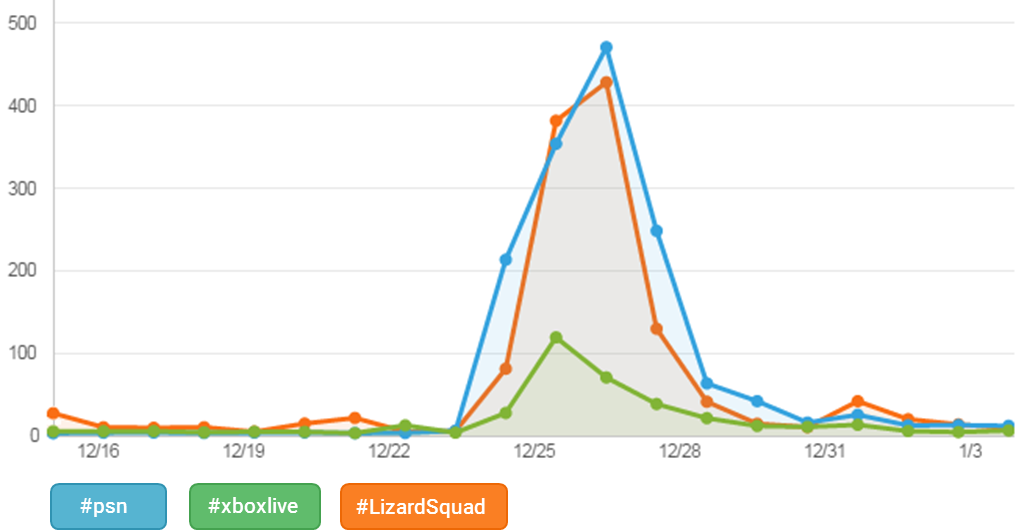
\includegraphics[width=\textwidth]{final_timeseries_psnhack}
  \caption[Christmas Network Outage Word Cloud]{Christmas Network Outage Word Cloud}
  \label{fig:christmas-network-outage-word-cloud}
  \vspace{-1.3em}
\end{figure}

Naaman et al. used twitter to \enquote{identify important dimensions according to which trends can be categorized, as well as the key distinguishing features of trends that can be derived from their associated messages} \cite{naaman2011characterizing}. They performed their analysis on previously collected dataset of 48 million tweets while we try to achieve results on a much smaller dataset and with live data instead of historic data. Zubiaga et al. focus on the classification problem by \enquote{introducing a typology of trending topics, and providing a method to immediately classify trending topics as soon as they  appear  on  the  homepage  of  Twitter} \cite{zubiaga2011classifications}. We however try to identify trends without knowing that Twitter declared them as trending.



\section{Setup / Limitations}
\label{sec:setup}
\todo[inline]{decide on section title}
For this case study, Twitter is used as the only data source. However, other social media sources for additional public social data could easily be integrated into the current data flow. This case study is limited to only collecting tweets in English language since NLP in English is more advanced, offers a proper comparison and is simpler to use. In addition, the Twitter Streaming API is restricted to 1\% of the total number of Tweets at any given moment\footnote{\url{http://dev.twitter.com/docs/faq} \accessednote}.

The use of commercial sentiment analysis API's would be too expensive for this huge number of Tweets. Therefore, we utilized free machine learning technologies for this task. However, only the first five million Tweets have been classified with a sentiment by machine learning techniques due to the expensive computing power that is required for such a huge data set. We restricted our analysis not only on tweets in English but also to tweets from anywhere in the United States of America. This makes it easier to use geospatial visualisations techniques.


\section{Analysis Methods}
\label{sec:technologies}
Mining, storing, analyzing and visualizing terabytes of unstructured data requires optimized and new cutting edge technologies. 

Since traditional relational \textbf{databases} cannot meet these requirements \cite{TwitterDataAnalytics2013}, new NoSQL databases\footnote{NoSQL ('Not Only SQL') represents a new type of data management technologies created to meet the new requirements to process, store and analyze Big Data.} had been invented, such as MongoDB\footnote{\url{http://www.mongodb.org} \accessednote }, Apache Cassandra\footnote{\url{http://cassandra.apache.org} \accessednote} and CouchDB\footnote{\url{http://couchdb.apache.org} \accessednote}, that makes it possible to store, manage and analyze the huge amount of unstructured data in real time. Further optimization can be achieved by using Apache Hadoop\footnote{\url{http://hadoop.apache.org} \accessednote} to distribute the data storage and processing across machine clusters.


\subsection{Data Preparation}
\label{subsec:data-preparation}
\textbf{Natural Language Processing} is an important part of the analysis of big social data. Toolkits such as Python NLTK\footnote{\url{http://nltk.org} \accessednote} and Apache OpenNLP\footnote{\url{http://opennlp.apache.org} \accessednote} offer a rich set of algorithm for tokenization, stemming, named entity recognition, stop word removal and more.

\textbf{Stop word removal} describes the process of removing the most common words out of a text. Words like \textit{to}, \textit{the} or \textit{a} have little influence in any analysis and are most of the time omitted to avoid unnecessary indices and clean the dataset. Normally so called \textit{stop lists} are defined containing all words which should be removed before the analysis \cite[27]{manning2008introduction}. However in some cases it can be dangerous or simply wrong to remove too many stop words or to remove stop words at all. For example when searching for some \enquote{well known pieces of verse consist entirely of words that are commonly on stop lists (To be or not to be, Let It Be, I don’t want to be, ... )} \cite[27]{manning2008introduction}.

\textbf{Stemming} is used to bring related terms and words to a common base form. This is often needed when texts are analysed and words in different forms are used like \textit{am}, \textit{are} or \textit{is} a stemming algorithm would then find the common base form as \textit{be}. There exist different approaches for stemming like just cutting off the ends of words and hoping for a good result. More advanced approaches try to find the correct base \enquote{with the use of a vocabulary and morphological analysis of words, normally aiming to remove inflectional endings only} \cite[32]{manning2008introduction}.

A \textbf{bag of words model} describes a technique where documents are analysed by counting and weighting their words. Each word can be a so called bag. The technique can be further enhanced to include weighting of words, for example stop words should have less weight. Another approach is to use a stemming algorithm on each word in order reduce the amount of bags. A bag of words model is much simpler than applying topic modelling algorithms described in the next section and therefore more convenient in some cases. \cite[117]{manning2008introduction}


\subsection{Sentiment Analysis}
\label{subsec:sentiment-analysis}
Sentiment Analysis is a widely used NLP technique to analyze social media data. Therefore, many companies, such as AlchemyAPI\footnote{\url{http://alchemyapi.com} \accessednote}, ViralHeat\footnote{\url{http://viralheat.com} \accessednote} and TextAlytics\footnote{\url{http://textalytics.com} \accessednote}, offer commercial web services to detect sentimental information of any text data by utilizing machine learning techniques. Several open-source machine learning toolkits, e.g. Weka\footnote{\url{http://cs.waikato.ac.nz/ml/weka} \accessednote} and Mallet\footnote{\url{http://mallet.cs.umass.edu} \accessednote}, offer similar algorithm that can be trained to classify and compute the corresponding sentiment. Further, these libraries are also suited for topic modeling, information extraction and pattern recognition on big social data. Apache UIMA\footnote{\url{http://uima.apache.org} \accessednote} and Gate\footnote{\url{http://gate.ac.uk} \accessednote} provide extensible frameworks to combine and manage these technologies for the analysis of unstructured information.
\todo[inline]{Insert figure and reference it}


\subsection{Topic Modelling}
\label{subsec:topic-modelling}
\todo[inline]{add correct citations}
Topic modeling is a statistical machine learning model for automatic discovery of abstract topics occurring in a collection of documents (content entities). Moreover, it allocates the analyzed documents to the discovered topics and clusters the most common words (terms). \acf{LDA} is a common method of topic modeling introduced by Blei et al. [BNJ03]. The \ac{LDA} method assumes that each document contains a mixture of topics where each word attributes to one of these topics [BNJ03]. The requirements for executing \ac{LDA} for topic modelling are a collection of documents, a specified number of topics and specified number of iterations. A highly simplified process description of LDA is described below:
\begin{enumerate}
  \item{Go through every document and assign a random topic (from the specified number of topics) to each word occurrence}
  \item{Count up the number of assignments of each word occurrence for every topic (how many times for each topic does a word appear)}
  \item{Resemble the topic assignment for one selected word occurrence in a document:}
  \begin{itemize}
    \item{Delete the assignment of the selected word occurrence}
    \item{Compute conditional distribution over all possible topic assignment of the selected word:}
    \begin{itemize}
      \item{A = number of assigned word occurrence categorized by their topics for the document}
      \item{B = number of times each topic appeared in the document}
      \item{C = number of assignments of each word for every topic}
      \item{(A+B)*C = topic with highest value is new topic assignment for the selected word occurrence}
    \end{itemize}
  \end{itemize}
  \item{Repeat with step two for the specified number of iterations}
\end{enumerate}
When analyzing detected trends on twitter we utilize \ac{LDA} to find all topics related to hashtags. The documents needed for \ac{LDA} are in this case the collected tweets and the parameters topic count and iteration count are varied depending on the trend. Ramage et al. find in their research paper that the 140 characters of a tweet are sufficient as a document for \ac{LDA} \cite{ramage2010lda}.
\todo[inline]{Insert figure and reference it}


\subsection{Visualization}
\label{subsec:visualization}
To understand and interpret the results of this big social data analysis, we used a variety of visualization techniques that help to get valuable insights about certain aspects.

\subsubsection{Time Series}
\label{subsubsec:vis-time-series}
The time series visualization is used to display the course of an event or a trend. It displays the dates in which the trend has been monitored on the horizontal axis against the count of tweets collected for that topic on the vertical axis. The time series evaluation are particularly good when it comes to detecting new trends. Most trending topics will not show up in previous data at all but as soon as they begin to trend they show as clear peaks in the times series graph.
\todo[inline]{Insert figure and reference it}
Figure XX shows a time series visualization of the hashtags \textit{XXX} and \textit{XXX}. There is an observable peak of both hashtags on XXXXXXXXXX which is very hard to spot when solely looking at the data without any visualization. The big advantage of the time series visualization over the other visualization techniques is that it considers the time. That allows us to see when a topic begins to trend.

\subsubsection{Word Clouds}
\label{subsubsec:vis-word-clouds}
The word cloud visualization highlights the most frequently occurring terms in the current twitter activity related to a trending topic. Thereby, the importance of a term is expressed using its font size. This visualization type is known as an effective summarizing technique and helps to detect the related topics to a trend.

The current implementation uses all tweets related to a trend and transforms them into a word cloud. Therefore all tweets are read from the database and then the frequency of each word in the text is counted using wordfreq.js\footnote{\url{http://timdream.org/wordfreq} \accessednote}. Finally, every unique word and the associated frequency is forwarded to wordcloud2.js\footnote{\url{http://timdream.org/wordcloud2.js} \accessednote}, a JavaScript visualization library, to render the corresponding word cloud.

\todo[inline]{Insert figure and reference it}

An example word cloud is depicted in figure XXX. ABCDE and FGHIJK are the most common terms for the detected trend

\subsubsection{Geospatial Visualization}
\label{subsubsection:vis-geospatial}
Geospatial visualization helps to identify the location of current events and detect new events and trends that are likely to occur \cite{TwitterDataAnalytics2013}. Furthermore, it is used to gain insights into the prominent locations discussing a selected event \cite[64-66]{TwitterDataAnalytics2013}. As mentioned in section \ref{sec:setup}, the geospatial visualization is limited only to English and geolocated Tweets. All visualizations are build with CartoDB\footnote{\url{http://cartodb.com} \accessednote}, a cloud-computing platform that provides mapping and visualization solutions for geolocated data. 

\todo[inline]{Insert figure and reference it}

Lorem ipsum figure XXX describes flow of topic around the usa with major impact in new york ....


\section{Architecture}
\label{sec:architecture}
The Twitter Stream Reader is implemented with Python using the Twython\footnote{\url{http://twython.readthedocs.org} \accessednote} library to access the Twitter Streaming API\footnote{Push service to collect public Tweets in realtime.}. The streaming data from Twitter is filtered based on \todo{finish sentence!}. A Tweet contains a 140 character text message and various metadata such as the language, location, user information, number of retweets and favorites and more. 

\todo{Check if following fits into our setup}
The language used in Tweets is mostly informal and the correctness of grammar is often sacrificed to gain additional characters. Further, abbreviations and special characters (e.g. emoticons) are also frequently employed \cite[67]{TwitterDataAnalytics2013}. Therefore, each Tweet is preprocessed in the Data Analysis Module using common NLP text preparation techniques to remove these elements. In the first step, the text of a Tweet is lowercased and special characters, URLs as well as English stop words\footnote{Words that do not contain important significance or are extremely common (e.g. the, a, want).} get removed.

\todo{Fit paragraph into text}
In the next step, the preprocessed Tweet text alongside with the original Tweet text, creation timestamp and all metadata is stored into MongoDB, a popular NoSQL database that is used as the main data store for our implementation.
